\chapter{La conoscenza}\index{conoscenza}
\section{Introduzione}
Il cuore dei sistemi complessi, umani e artificiali, è nella conoscenza che essi sono in grado di mettere a disposizione dei processi che fanno funzionare il sistema stesso. La conoscenza è indispensabile per percepire l’ambiente esterno, modificare gli stati interni, costruire piani e agire nel mondo. Fin dall’antichità è stata colta l’importanza della conoscenza («sapere è potere»), ma solo recentemente si è preso coscienza del fatto che è anche determinante la capacità di \emph{usare} la conoscenza.

\begin{figure}[hbt]
  \centering
  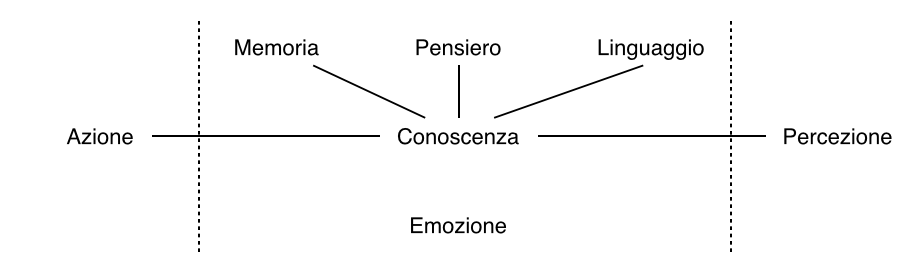
\includegraphics[width=\textwidth]{img/conoscenza.png}
  \caption{La conoscenza}
  \label{fig:conoscenza}
\end{figure}

Con il tempo sono aumentati gli strumenti per immagazzinare e acquisire conoscenza; ciò che diversifica è saper usare, gestire e scremare la conoscenza secondo i propri scopi. Conoscenza, memoria e apprendimento sono strettamente collegati e fanno parte degli stessi processi mentali, dato che corrispondono a modi diversi di considerare gli stessi fenomeni, analizzati da prospettive differenti e con scopi differenti.

Analizzare la conoscenza umana prevede diversi interrogativi su: qualità della conoscenza, rappresentazione, gestione, apprendimento.

\section{Tipi di conoscenza}
Nel tracciare una mappa della struttura della conoscenza umana si utilizza una divisione in tre sottoinsiemi interagenti, che gestiscono ciascuno un tipo di conoscenza: \emph{esplicita}, \emph{tacita} e \emph{modellistica} (k sta per ``knowledge'').

\begin{figure}[hbt]
  \centering
  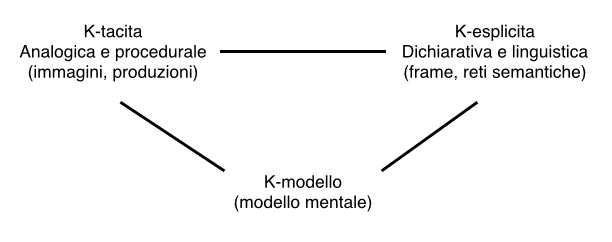
\includegraphics[width=0.9\textwidth]{img/k-conoscenza.png}
  \caption{Suddivisione della conoscenza}
  \label{fig:kconoscenza}
\end{figure}

La conoscenza esplicita\index{conoscenza!esplicita} è una teoria del mondo concepita come un insieme di entità concettuali che descrivono proposizionalmente classi di oggetti (il bicchiere), relazioni (il vino sta dentro al bicchiere), processi (la maturazione dell’uva), regole ufficiali di comportamento (non si beve con la bocca piena), ecc. È tipicamente rappresentabile con un formalismo logico. La conoscenza esplicita rappresenta ciò che una persona sa di sapere intorno a qualunque entità del mondo. È la conoscenza consapevole, esprimibile linguisticamente, su cui si può volontariamente riflettere. Non è detto che tale conoscenza corrisponda effettivamente alla realtà esterna, ma corrisponde a quello che la persona crede sia la realtà esterna.

La conoscenza tacita\index{conoscenza!tacita} si riferisce alla conoscenza che un sistema possiede e che gli permette di interagire efficacemente con il mondo, pur non essendo rappresentata in modo esplicito. Il modo standard di rappresentarla è attraverso le regole di produzione. La parte \emph{trasparente} di k-tacita corrisponde alle immagini e alle produzioni, che traducono in termini procedurali la conoscenza esplicita, determinando il cambiamento dello stato del mondo. La parte \emph{opaca} invece è costituita dai modi di agire che scattano automaticamente, senza bisogno di controllo o attenzione (e.g. andare in bici, distinguere gli aromi). Sono per definizione fuori dalla consapevolezza: agiscono inconsciamente e sono ricostruibili solo a posteriori.

La conoscenza tacita corrisponde a saper agire in una determinata situazione ed è quindi sovrapponibile alla conoscenza procedurale\index{conoscenza!procedurale}, tipica dei casi in cui una persona sa come agire ma non sa come esplicitare cosa ha attivato la reazione adatta a quella situazione. Il caso più frequente è quando si sa cosa si sta facendo, ma non è facile verbalizzarlo (e.g. un chirurgo che sa operare ma non sa spiegare facilmente come ha mosso le mani per farlo).

Queste caratteristiche hanno fatto ipotizzare che non si possa parlare di conoscenza, ma piuttosto di \emph{background capacities}, attualmente non rappresentabili con i metodi odierni.

La relazione tra k-tacita e k-esplicita è complessa e sfuggente. Di una conoscenza tacita si può tentare di inferire quale possa essere il corrispettivo esplicito, che corrisponde a costruire la teoria di un fenomeno, con il fenomeno introspettivo invece che appartiene al mondo esterno. Come dalla conoscenza tacita si può arrivare a costruire una teoria proposizionale, così dalla conoscenza esplicita si può strutturare una conoscenza procedurale.

La conoscenza modello (k-modello)\index{conoscenza!modello} è un modello specifico costruito integrando i due precedenti tipi di conoscenza che abbiamo già visto. Può essere considerata come un insieme di configurazioni parziali della conoscenza teorica espressa da k-esplicita e k-tacita. Il modo standard di rappresentarla è attraverso i \emph{modelli mentali}\index{modelli mentali}, che riuniscono dati e procedure, saper che cosa e sapere come. Il k-modello costituisce quindi la parte di conoscenza che il sistema sta effettivamente adoperando in un momento dato.

\section{Chunking}\index{chunking}
Il \emph{chunk} è un'unità di informazione. L'operazione di acquisizione di queste unità è chiamata chunking.

 Per Clayton Lewis\index{Lewis, Clayton} (1978) il chunk è quell'insieme strutturato d'informazioni immagazzinate nel momento in cui la conoscenza viene acquisita. Di fronte ad una nuova situazione, si impara il relativo chunk d'informazioni; il chunk acquisito descrive quella situazione e la risposta da noi prodotta, cosicché al verificarsi di situazioni analoghe la risposta sarà sempre più immediata e precisa.

La conoscenza è in primis immagazzinata in forma \emph{dichiarativa}, poi progressivamente trasformata in conoscenza \emph{procedurale}, e quindi consolidata in chunk sempre più complessi. Ad esempio, dalla conoscenza dichiarativa di come si gira il volante, si passa alla conoscenza procedurale di come si fa a guidare (e non sarà più necessaria un'attenzione attiva per riuscire a svolgere questo compito) e quindi al controllo sempre più pieno e preciso dell'autovettura (dovuto alla formazione di un chunk via via più complesso).

\section{Rappresentazione della conoscenza}\index{rappresentazione della conoscenza}
La rappresentazione della conoscenza è una branca dell'intelligenza artificiale che studia il modo in cui avviene il ragionamento umano, e si preoccupa di definire dei simbolismi o dei linguaggi che permettano di formalizzare la conoscenza al fine di renderla comprensibile alle macchine, per potervi fare dei ragionamenti automatici (inferendo le informazioni presenti) ed estrarre così nuova conoscenza.

Un punto chiave della rappresentazione della conoscenza è la definizione di linguaggi che siano sufficientemente espressivi da permettere di descrivere il dominio di interesse, ma non troppo ricchi di espressività, in quanto richiederebbero troppe risorse, troppo tempo per applicarvi i meccanismi inferenziali, o peggio ancora entrambi.

In linea generale, i linguaggi di rappresentazione della conoscenza forniscono sia una serie di costrutti per definire la sintassi del dominio di interesse (le regole sulle quali costruire delle asserzioni accettabili), sia una serie di operatori (quantificatori, operatori modali, ecc) che permettano di dare un significato, un valore di verità alle asserzioni rispetto al modello di riferimento.

Attraverso il linguaggio scelto si andranno ad effettuare una serie di asserzioni sul mondo, che andranno insieme a costituire una \emph{base di conoscenza}\index{base di conoscenza} (o kowledge base, KB). È inoltre importante che il linguaggio scelto per fare le asserzioni sia anche in grado di operare sulla KB per estrarre nuova conoscenza e per aggiungerne di nuova.

Esistono principalmente due metodologie per rappresentare la conoscenza: i \emph{linguaggi formali} e gli \emph{alberi di decisione}.

\section{Intelligenza emotiva}\index{intelligenza emotiva}
L'intelligenza emotiva è un aspetto dell'intelligenza legato alla capacità di riconoscere, utilizzare, comprendere e gestire in modo consapevole le proprie ed altrui emozioni. Viene definita come la capacità di controllare i sentimenti ed emozioni proprie ed altrui, distinguere tra di esse e di utilizzare queste informazioni per guidare i propri pensieri e le proprie azioni.
\subsection{Consapevolezza di sé}
La consapevolezza di sé comporta la conoscenza dei propri stati interiori, preferenze, risorse e intuizioni. Può essere raggiunta tramite consapevolezza emotiva, ovvero il riconoscimento delle proprie emozioni e dei loro effetti, l’autovalutazione accurata, ovvero conoscere i propri punti di forza e i propri limiti, la fiducia in sé stessi, ovvero la sicurezza nel proprio valore e nelle proprie capacità.
\subsection{Padronanza di sé}
La padronanza di sé è la capacità di dominare gli stati interiori, gli impulsi e le risorse. Si compone di autocontrollo (dominio delle emozioni e degli impulsi distruttivi), fidatezza, (mantenimento di standard di onestà e integrità), coscienziosità (assunzione delle responsabilità per quanto attiene alla propria prestazione), adattabilità (flessibilità nel gestire il cambiamento), innovazione (capacità di sentirsi a proprio agio e di avere un atteggiamento aperto di fronte a idee, approcci e informazioni nuovi).
\subsection{Motivazione}
La motivazione comporta tendenze emotive che guidano o facilitano il raggiungimento di obiettivi: spinta alla realizzazione (impulso a migliorare o a soddisfare uno standard di eccellenza), impegno (adeguamento agli obiettivi del gruppo o dell’organizzazione), iniziativa (prontezza nel cogliere le occasioni), ottimismo (costanza nel perseguire gli obiettivi nonostante ostacoli e insuccessi).
\subsection{Empatia}
L’empatia comporta la consapevolezza dei sentimenti, delle esigenze e degli interessi altrui: comprensione degli altri (percezione dei sentimenti e delle prospettive altrui; interesse attivo per le preoccupazioni degli altri), assistenza (anticipazione, riconoscimento e soddisfazione delle esigenze del cliente), promozione dello sviluppo altrui (percezione delle esigenze di sviluppo degli altri e capacità di mettere in risalto e potenziare le loro abilità), sfruttamento della diversità (saper coltivare le opportunità offerte da persone di diverso tipo).
\subsection{Abilità sociali}
Le abilità sociali comportano abilità nell'indurre risposte desiderabili negli altri. Si caratterizza in influenza (impiego di tattiche di persuasione efficienti), comunicazione (invio di messaggi chiari e convincenti), leadership (capacità di ispirare e guidare gruppi), catalisi del cambiamento (capacità di iniziare o dirigere il cambiamento),  gestione del conflitto (capacità di negoziare e risolvere situazioni di disaccordo), costruzione di legami (capacità di favorire e alimentare relazioni utili) collaborazione e cooperazione (capacità di lavorare con altri verso obiettivi comuni), lavoro in team (capacità di creare una sinergia di gruppo nel perseguire obiettivi comuni), consapevolezza politica (saper leggere e interpretare le correnti emotive e i rapporti di potere in un gruppo).

Tali constatazioni hanno portato poco per volta al riconoscimento che l'intelligenza basata sull'esercizio della pura razionalità costituisce soltanto un aspetto delle più generali capacità che permettono all'uomo di misurarsi con le diverse situazioni incontrate nella vita di tutti i giorni e di risolvere adeguatamente i problemi che esse implicano. Questo orientamento sembrerebbe essere confermato anche su un piano prettamente neurofisiologo.